\de{ĐỀ THI HỌC KỲ I NĂM HỌC 2022-2023}{TRƯỜNG THPT Trương Vĩnh Ký - Bến Tre}

\begin{center}
	\textbf{PHẦN 1 - TRẮC NGHIỆM}
\end{center}
\Opensolutionfile{ans}[ans/ans]
\begin{ex}%Câu 1%[0D1Y1-1]%[Dự án đề kiểm tra HKII NH22-23- Trường THPT Trương Vĩnh Kỹ]%[GV: Nguyễn Tài Tuệ]
	Phát biểu nào sau đây là một mệnh đề?
	\choice
	{Trời hôm nay đẹp quá!}
	{\True New York là thủ đô của Việt Nam}
	{Con đang làm gì đó?}
	{Số $ 3 $ có phải là số tự nhiên không?}
	\loigiai{
		Khẳng định \lq\lq New York là thủ đô của Việt Nam\rq\rq~ là một mệnh đề.
	}
\end{ex}

\begin{ex}%Câu 2%[0D1Y1-2]%[Dự án đề kiểm tra HKII NH22-23- Trường THPT Trương Vĩnh Kỹ]%[GV: Nguyễn Tài Tuệ]
	Trong các câu sau, câu nào là mệnh đề đúng?
	\choice
	{Hãy ngồi trật tự!}
	{Sách này có mấy chương?}
	{\True $ 7 $ là số nguyên tố}
	{$ 15 $ là số tự nhiên chẵn}
	\loigiai{
		Mệnh đề \lq\lq $ 7 $ là số nguyên tố\rq\rq~ là một mệnh đề đúng.
	}
\end{ex}

\begin{ex}%Câu 3%[0D1Y1-5]
	Mệnh đề phủ định của mệnh đề  \lq\lq~$\exists x \in \mathbb{R}\colon x^2+x+1 \leq 0$\rq\rq~ là
	\choice
	{\lq\lq~$\exists x \in \mathbb{R}\colon x^2+x+1>0$\rq\rq~}
	{\lq\lq~$\forall x \in \mathbb{R}\colon x^2+x+1 \leq 0$\rq\rq~}
	{\True \lq\lq~$\forall x \in \mathbb{R}\colon x^2+x+1>0$\rq\rq~}
	{\lq\lq~$\forall x \in \mathbb{R}\colon x^2+x+1 \geq 0$\rq\rq~}
	\loigiai{
	Mệnh đề phủ định của mệnh đề \lq\lq~$\exists x \in \mathbb{R}\colon x^2+x+1 \leq 0$\rq\rq~ là \lq\lq~$\forall x \in \mathbb{R}\colon x^2+x+1>0$\rq\rq~.
	}
\end{ex}

\begin{ex}%Câu 4%[0D1B2-1]%[Dự án đề kiểm tra HKII NH22-23- Trường THPT Trương Vĩnh Kỹ]%[GV: Nguyễn Tài Tuệ]
	Liệt kê phần tử của tập hợp $B=\left\{x \in \mathbb{N}\mid\left(2 x^2-x\right)\left(x^2-3 x-4\right)=0\right\}$ là
	\choice
	{$B=\{-1 ; 0 ; 4\}$}
	{\True $B=\{0 ; 4\}$}
	{$B=\left\{-1 ; \dfrac{1}{2}; 0 ; 4\right\}$}
	{$B=\{0 ; 1 ; 4\}$}
	\loigiai{
		Ta có $ \left(2 x^2-x\right)\left(x^2-3 x-4\right)=0\Leftrightarrow \hoac{&2x^2-x=0\\&x^2-3x-4=0}\Leftrightarrow \hoac{&x=0\\&x=\dfrac{1}{2}\\&x=-1\\&x=4.}$\\
		Vì $ x\in \mathbb{N}\Rightarrow B=\{0,4\} $.
	}
\end{ex}

\begin{ex}%Câu 5%[0D1B2-2]%[Dự án đề kiểm tra HKII NH22-23- Trường THPT Trương Vĩnh Kỹ]%[GV: Nguyễn Tài Tuệ]
	Số tập con gồm ba phần tử của tập hợp $\{1 ; 2 ; 3 ; 4 ; 5\}$ là
	\choice
	{$ 8  $}
	{$ 12  $}
	{$ 7  $}
	{\True $ 10  $}
	\loigiai{
		Các tập con của tập $\{1 ; 2 ; 3 ; 4 ; 5\}$ là\\
		$ A_1=\{1;2;3\}$, $A_2=\{1;2;4\}$,  $ A_3=\{1;2;5\} $, $ A_4=\{1;3;4\} $, $ A_5=\{1;3;5\}$, $A_6=\{1;4;5\} $, $ A_7=\{2;3;4\} $, $ A_8=\{2;3;5\} $, $ A_9=\{2;4;5\} $, $ A_{10}=\{3;4;5\} $.\\
		Số tập con gồm $ 3 $ phần tử là $ 10 $.
	}
\end{ex}

\begin{ex}%Câu 6%[0D1B3-1]%[Dự án đề kiểm tra HKII NH22-23- Trường THPT Trương Vĩnh Kỹ]%[GV: Nguyễn Tài Tuệ]
	Cho hai tập hợp $A=\{1 ; 2 ; 3 ; 4\}, B=\{2 ; 4 ; 6 ; 8\}$. Tập hợp $A \cap B$ là
	\choice
	{\True $\{2 ; 4\}$}
	{$\{1 ; 2 ; 3 ; 4 ; 6 ; 8\}$}
	{$\{6 ; 8\}$}
	{$\{1 ; 3\}$}
	\loigiai{
	Ta có $A \cap B = \{2 ; 4\}$.
	}
\end{ex}

\begin{ex}%Câu 7%[0D1B3-4]%[Dự án đề kiểm tra HKII NH22-23- Trường THPT Trương Vĩnh Kỹ]%[GV: Nguyễn Tài Tuệ]
	Tập $(-\infty ;-3) \cap[-5 ; 2)$ bằng
	\choice
	{\True$[-5 ;-3)$}
	{$(-\infty ;-5]$}
	{$(-\infty ;-2)$}
	{$(-3 ;-2)$}
	\loigiai{
	Ta có $(-\infty ;-3) \cap[-5 ; 2) =[-5 ;-3)$.
	}
\end{ex}

\begin{ex}%Câu 8%[0D1B3-3]%[Dự án đề kiểm tra HKII NH22-23- Trường THPT Trương Vĩnh Kỹ]%[GV: Nguyễn Tài Tuệ]
	Lớp 10A có $ 30 $ học sinh giỏi, trong đó có $ 15 $ học sinh giỏi môn Toán, $ 20 $ học sinh giỏi môn Ngữ Văn. Hỏi lớp 10A có tất cả bao nhiêu học sinh giỏi cả hai môn Toán và Ngữ văn?
	\choice
	{$ 30  $}
	{\True $ 5  $}
	{$ 15  $}
	{$ 10  $}
	\loigiai{
		Gọi $ x $ là số học sinh giỏi cả hai môn Toán và Ngữ văn.\\
		Ta có $ 15+20-x=30\Leftrightarrow x=5 $.\\
		Do đó có $ 5 $ học sinh giỏi cả hai môn Toán và Ngữ văn.
	}
\end{ex}

\begin{ex}%Câu 9%[0D2Y1-1]%[Dự án đề kiểm tra HKII NH22-23- Trường THPT Trương Vĩnh Kỹ]%[GV: Nguyễn Tài Tuệ]
	Cặp số $(-2 ; 3)$ là nghiệm của bất phương trình nào dưới đây?
	\choice
	{$2 x+y+1>0$}
	{$x+3 y+1<0$}
	{$2 x-y-1 \geq 0$}
		{\True $x+y+1>0$}
	\loigiai{
		Ta thấy cặp số $ (-2;3)  $ thỏa mãn bất phương trình $  x+y+1>0 $.
	}
\end{ex}

\begin{ex}%Câu 10%[0D2B1-2]%[Dự án đề kiểm tra HKII NH22-23- Trường THPT Trương Vĩnh Kỹ]%[GV: Nguyễn Tài Tuệ]
\immini{	Miền không gạch sọc trong hình vẽ là hình biểu diễn miền nghiệm của bất phương trình nào sau đây?
	\choice
	{$2 x-y+1 \geq 0$}
	{$x+2 y-2 \leq 0$}
	{$x+2 y+1 \leq 0$}
	{\True $x+2 y-2 \geq 0$}}{\begin{tikzpicture}[line join=round, line cap=round,>=stealth,thick]
		\tikzset{every node/.style={scale=0.9}}
		\begin{scope}
			\clip (-2,-1) rectangle (3,2.5);
			\fill[pattern=north east lines] (-4,3)--(-4,-1.5)--(5,-1.5)--cycle;
			\draw (-3,2.5)--(4,-1) node [pos=0.45, above, sloped] { };
		\end{scope}
		\draw[->] (-2,0)--(3,0) node[below]{$x$};
		\draw[->] (0,-1)--(0,2.5) node[left]{$y$};
		\draw (0,0) node[below left]{$O$};
		\foreach \x in {2}
		\draw[thin] (\x,1pt)--(\x,-1pt) node [above] {$\x$};
		\foreach \y in {1}
		\draw[thin] (1pt,\y)--(-1pt,\y) node [above right] {$\y$};
\end{tikzpicture}}
\loigiai{
	Bờ của miền nghiệm  là đường thẳng đi qua hai điểm $ (0;1) $ và $ (2;0) $ có phương trình $$ x+2y-2=0.$$
	Điểm $ O(0,0) $ không thuộc miền nghiệm. \\
	Do đó chỉ có bất phương trình $x+2 y-2 \geq 0$ thỏa mãn.
}
\end{ex}

\begin{ex}%Câu 11%[0D2B1-3]%[Dự án đề kiểm tra HKII NH22-23- Trường THPT Trương Vĩnh Kỹ]%[GV: Nguyễn Tài Tuệ]
	Bạn Minh Diệp làm một bài thi giữa kì $ 1 $ môn Toán. Đề thi gồm $ 35 $ câu hỏi trắc nghiệm và $ 3 $ bài tự luận. Khi làm đúng mỗi câu trắc nghiệm sẽ được $ 0,2 $ điểm, làm đúng mỗi câu tự luận được $ 1 $ điểm. Giả sử bạn Minh Diệp làm đúng $x$ câu hỏi trắc nghiệm và $y$ bài tự luận. Viết một bất phương trình bậc nhất hai ẩn $x$ và $y$ để đảm bảo bạn Minh Diệp được ít nhất $ 8 $ điểm.
	\choice
	{$0,2 x+y<8$}
	{\True $0,2 x+y \geq 8$}
	{$35 x+3 y \geq 8$}
	{$x+0,2 y \geq 8$}
	\loigiai{
		Số điểm trắc nghiệm bạn Minh Diệp đạt được là $ 0,2\cdot x $ điểm.\\
		Số điểm tự luận của bạn Minh Điệp đạt được là $ y $ điểm.\\
		Để bạn Minh Diệp được ít nhất $ 8 $ điểm thì $ 0,2x+y\ge 8 $.
	}
\end{ex}

\begin{ex}%Câu 12%[0H1Y1-2]%[Dự án đề kiểm tra HKII NH22-23- Trường THPT Trương Vĩnh Kỹ]%[GV: Nguyễn Tài Tuệ]
	Giá trị của $\tan 30^{\circ}$ là
	\choice
	{\True$\dfrac{\sqrt{3}}{3}$}
	{$-\dfrac{\sqrt{3}}{3}$}
	{$\sqrt{3}$}
	{$-\sqrt{3}$}
	\loigiai{
		Ta có $ \tan 30^\circ =\dfrac{\sqrt{3}}{3}$.
	}
\end{ex}

\begin{ex}%Câu 13%[0H1B2-1]%[Dự án đề kiểm tra HKII NH22-23- Trường THPT Trương Vĩnh Kỹ]%[GV: Nguyễn Tài Tuệ]
	Cho $\triangle A B C$ có $A B=4$, $A C=6$, $\widehat{A}=120^{\circ}$. Độ dài cạnh $B C$ bằng
	\choice
	{$\sqrt{19}$}
	{$3 \sqrt{19}$}
	{\True $2 \sqrt{19}$}
	{$2 \sqrt{7}$}
	\loigiai{
	Ta có $ BC=\sqrt{AB^2+AC^2-2AB\cdot AC\cdot \cos A}=\sqrt{4^2+6^2-2\cdot 4\cdot 6 \cdot \cos 120^\circ}=2\sqrt{19} $.
	}
\end{ex}

\begin{ex}%Câu 14%[0H1B2-1]%[Dự án đề kiểm tra HKII NH22-23- Trường THPT Trương Vĩnh Kỹ]%[GV: Nguyễn Tài Tuệ]
	Cho tam giác $A B C$ có $A B=5 ; \widehat{A}=30^{\circ}; \widehat{B}=70^{\circ}$. Độ dài của cạnh $B C$ có giá trị gần nhất với giá trị nào dưới đây?
	\choice
	{$ 5,2  $}
	{\True$ 2,5  $}
	{$ 2,6  $}
	{$ 9,8  $}
	\loigiai{
	Ta có $ \widehat{C}=180^\circ-30^\circ-70^\circ =80^\circ $.\\
	Áp dụng định lý sin ta có
	$ \dfrac{BC}{\sin A}=\dfrac{AB}{\sin C}\Rightarrow BC=\dfrac{AB\cdot \sin A}{\sin C}\approx 2,5$.
	}
\end{ex}

\begin{ex}%Câu 15%[0H1B2-2]%[Dự án đề kiểm tra HKII NH22-23- Trường THPT Trương Vĩnh Kỹ]%[GV: Nguyễn Tài Tuệ]
	Cho tam giác $A B C$ có $a=4, c=5, \widehat{B}=150^{\circ}$. Tính diện tích tam giác $A B C$.
	\choice
	{$ 10  $}
	{$10 \sqrt{3}$}
	{\True $ 5  $}
	{$5 \sqrt{3}$}
	\loigiai{
		Diện tích tam giác $ ABC $ là $ S=\dfrac{1}{2}ac\sin B= 5$.
	}
\end{ex}

\begin{ex}%[0H1K3-2]%[Dự án đề kiểm tra HKII NH22-23- Trường THPT Trương Vĩnh Kỹ]%[GV: Nguyễn Tài Tuệ]
\immini{
	Trên ngọn đồi có một tháp cao $100$ m (hình vẽ bên). Đỉnh tháp $B$ và chân tháp $C$ nhìn điểm $A$ ở chân đồi dưới một góc tương ứng $30^{\circ}$ và $60^{\circ}$ so với phương thẳng đứng. Xác định chiều cao $CH$ của ngọn đồi.
	\choice
	{$45$m}
	{$60$m}
	{\True $50$m}
	{$40$m}
}
{	
	\begin{tikzpicture}[scale=0.7, line join=round, line cap=round]
		\path 
		(0,0) coordinate (H)
		(0,2.5) coordinate (C)
		(0,7.5) coordinate (B)
		(4.33,0) coordinate (A)
		(1,0) coordinate (I)
		(-4,0) coordinate (K)
		;
		\draw[thick] (B)--(C);
		\draw (B)--(A)--(K)--(C)--(I) (C)--(H)  (C)--(A);
		\fill[pattern=north west lines] (C)--(I)--(K)--(C);			 
		\path (45:1.75) node[fill=white,inner sep=1pt]{$60^\circ$};
		\tkzMarkAngles[size=0.5cm](C,B,A)
			\draw		 
		 pic [draw,angle radius=2mm] {  angle = H--B--A}
		 pic [draw,angle radius=2mm] {  angle =H--C--A};
		  
		\path (85:5.6) node[fill=white,inner sep=1pt]{$30^\circ$};
		\foreach \p/\g in {A/-90,B/90,C/160,H/-90} \draw[fill] (\p) circle(.5pt)node [shift={(\g:.3)}] {$\p$};
	\end{tikzpicture}
}

\loigiai{
	Ta có $\widehat{BAC}=60^{\circ}-30^{\circ}=30^{\circ}$. (Áp dụng tính chất góc ngoài tam giác).\\
	Suy ra $\triangle ABC$ cân tại $C \Rightarrow AC=BC=100$ m.\\
	Xét $\triangle AHC$ có $\widehat{HAC}=30^{\circ} \Rightarrow HC=\dfrac{1}{2}AC=50$ m.}
\end{ex}
\begin{ex}%Câu 17%[0H2B1-2]%[Dự án đề kiểm tra HKII NH22-23- Trường THPT Trương Vĩnh Kỹ]%[GV: Nguyễn Tài Tuệ]
\immini{	Cho các véc-tơ $\vec{a}, \vec{b}, \vec{c}, \vec{u}$ và $\vec{v}$ như trong hình vẽ. Hỏi có bao nhiêu véc-tơ cùng hướng với véc-tơ $\vec{u}$ ?
	\choice
	{$ 4  $}
	{\True  $ 2  $}
	{$ 3  $}
	{$ 1  $}}{
	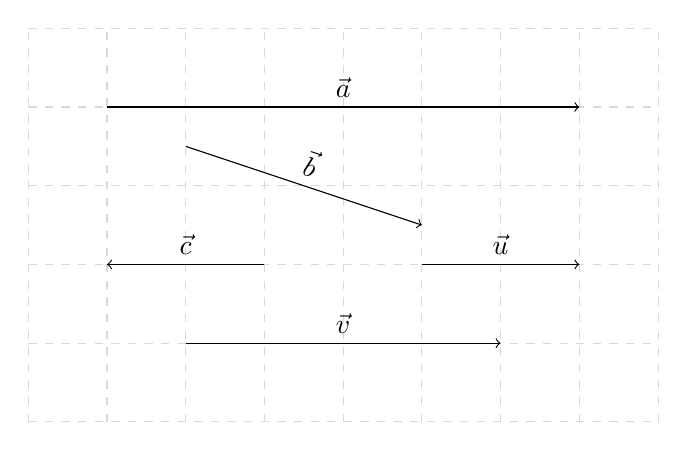
\begin{tikzpicture}
		\draw[dashed,gray!30] (0,0) grid (8,5);
		\draw[->] (2,1)--(6,1)node[pos=0.5,sloped,above]{$ \vec{v} $};
		\draw[->] (3,2)--(1,2)node[pos=0.5,sloped,above]{$ \vec{c} $};
		\draw[->] (5,2)--(7,2)node[pos=0.5,sloped,above]{$ \vec{u} $};
		\draw[->] (1,4)--(7,4)node[pos=0.5,sloped,above]{$ \vec{a} $};
		\draw[->] (2,3.5)--(5,2.5) node[pos=0.5,sloped,above]{$ \vec{b} $};
	\end{tikzpicture}}
\loigiai{
	Dựa khái niệm cùng hướng ta thấy $ \vec{u} $ cùng hương với các véc-tơ   $ \vec{v} $, $ \vec{a} $.
}
\end{ex}

\begin{ex}%Câu 18%[0H2Y2-1]%[Dự án đề kiểm tra HKII NH22-23- Trường THPT Trương Vĩnh Kỹ]%[GV: Nguyễn Tài Tuệ]
	Cho tam giác $A B C$, khẳng định nào sau đây là đúng?
	\choice
	{$\overrightarrow{A B}+\overrightarrow{A C}=\overrightarrow{B C}$}
	{\True $\overrightarrow{B C}+\overrightarrow{A B}=\overrightarrow{A C}$}
	{$\overrightarrow{A B}-\overrightarrow{A C}=\overrightarrow{B C}$}
	{$\overrightarrow{A B}+\overrightarrow{A C}=\overrightarrow{C B}$}
	\loigiai{
	Theo quy tắc cộng véc-tơ ta có $\overrightarrow{B C}+\overrightarrow{A B}=\overrightarrow{A B}+\overrightarrow{B C}=\overrightarrow{A C}$.
	}
\end{ex}

\begin{ex}%Câu 19%[0H2B2-6]%[Dự án đề kiểm tra HKII NH22-23- Trường THPT Trương Vĩnh Kỹ]%[GV: Nguyễn Tài Tuệ]
	Hai lực có giá đồng quy có độ lớn $F_1=F_2=10 \mathrm{~N}$, có $\left(\overrightarrow{F_1}, \overrightarrow{F_2}\right)=60^{\circ}$. Hợp lực của hai lực này có độ lớn gần nhất với giá trị nào sau đây?
	\choice
	{\True $17,3 \mathrm{~N}$}
	{$20 \mathrm{~N}$}
	{$14,1 \mathrm{~N}$}
	{$10 \mathrm{~N}$}
	\loigiai{
\immini{
Theo quy tắc hình bình hành ta có $ \vec{F}_1 +\vec{F}_2=\vec{AC}$ ( như hình vẽ).\\
Do $F_1=F_2=10 \mathrm{~N}$ và $\left(\overrightarrow{F_1}, \overrightarrow{F_2}\right)=60^{\circ}$ nên tam giác $ ABD $ là tam giác đều nên $ AO=\dfrac{AB\sqrt{3}}{2}\Rightarrow AC=AB\sqrt{3}=10\sqrt{3} $.\\
Mặt khác $ \vec{F}_1+\vec{F}_2=\vec{AC} $.\\
 Do đó hợp lực của hai véc-tơ $ \vec{F}_1 $, $ \vec{F}_2 $ bằng $ 10\sqrt{3}\approx 17.3$
	}{
	\begin{tikzpicture}
		\path 
		(0,0) node[rectangle,fill=blue!30,draw](A){A}
		($ (A)+(0:3) $)  coordinate (B)
		($ (A)+(60:3) $)  coordinate (D)
		($ (B)+(D)-(A) $) coordinate (C)
		(intersection of A--C and B--D) coordinate (O)
		;
		\draw[->](A)--(B)node[pos=0.5,sloped,above]{$ \vec{F}_1 $};
		\draw[->](A)--(C) ;
		\draw[->](A)--(D)node[pos=0.5,sloped,above]{$ \vec{F}_2 $};
		\draw (B)--(C)--(D) (B)--(D);
		\foreach \p/\g in {B/-90,C/0,D/90,O/-100} \draw[fill] (\p) circle(.5pt)node [shift={(\g:.3)}] {$\p$};
\end{tikzpicture}}
}
\end{ex}

\begin{ex}%Câu 20%[0H2Y3-1]%[Dự án đề kiểm tra HKII NH22-23- Trường THPT Trương Vĩnh Kỹ]%[GV: Nguyễn Tài Tuệ]
	\immini{Cho đoạn thẳng $A B$. Điểm $C$ thuộc đoạn $A B$ sao cho \break $3 A C=2 B C$.
	Chọn đẳng thức đúng.
	\choice
	{$2 \overrightarrow{A C}+3 \overrightarrow{C B}=\overrightarrow{0}$}
	{$2 \overrightarrow{A B}+5 \overrightarrow{A C}=\overrightarrow{0}$}
	{$5 \overrightarrow{A B}+2 \overrightarrow{C A}=\overrightarrow{0}$}
	{\True $2 \overrightarrow{A B}+5 \overrightarrow{C A}=\overrightarrow{0}$}
}{
	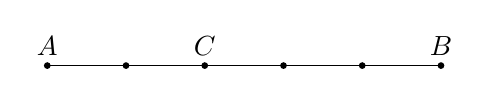
\begin{tikzpicture}
		\foreach  \i in {0,1,2,3,4,5}
		 \draw[fill=black] (\i,0) circle (1pt);
		 \draw (0,0)node[above]{$ A $}-- (2,0)node[above]{$ C $} --(5,0)node[above]{$ B $};
	\end{tikzpicture}}
\loigiai{
	 Dựa và khái niệm tích véc-tơ với một số ta có $2 \overrightarrow{A B}+5 \overrightarrow{C A}=\overrightarrow{0}$.
}
\end{ex}

\begin{ex}%Câu 21%[0H3Y1-3]%[Dự án đề kiểm tra HKII NH22-23- Trường THPT Trương Vĩnh Kỹ]%[GV: Nguyễn Tài Tuệ]
	Cho tam giác $A B C$ có $A(2 ; 1), B(-1 ; 0), C(1 ; 2)$. Tọa độ trọng tâm tam giác là
	\choice
	{$G(2 ; 1)$}
	{\True$G\left(\dfrac{2}{3}; 1\right)$}
	{$G=\left(\dfrac{2}{3}; \dfrac{1}{3}\right)$}
	{$G(1 ; 1)$}
	\loigiai{
		Ta có $ \heva{&x_G=\dfrac{x_A+x_B+x_C}{3}=\dfrac{2}{3}\\&y_G=\dfrac{y_A+y_B+y_C}{3}=1.} $\\
		Tọa độ trong tâm $G\left(\dfrac{2}{3}; 1\right)$.
	}
\end{ex}

\begin{ex}%Câu 22%[0H3B2-2]%[Dự án đề kiểm tra HKII NH22-23- Trường THPT Trương Vĩnh Kỹ]%[GV: Nguyễn Tài Tuệ]
	Trong mặt phẳng tọa độ $O x y$, cho hai vectơ $\vec{a}=(3 ; 2)$;  $\vec{b}=(5 ;-1)$. Tính góc giữa hai vectơ $\vec{a}$ và $\vec{b}$
	\choice
	{\True$45^{\circ}$}
	{$60^{\circ}$}
	{$90^{\circ}$}
	{$30^{\circ}$}
	\loigiai{
	Ta có $ \cos(\vec{a},\vec{b})=\dfrac{\vec {a}\cdot \vec{b}}{\left|\vec{a}\right |\cdot \left |\vec{b}\right|  }=\dfrac{13}{\sqrt{13}\cdot \sqrt{26}}=\dfrac{1}{\sqrt{2}}. $\\
	Do đó, góc giữa hai vectơ $\vec{a}$ và $\vec{b}$ là $ 45^\circ $.
	}
\end{ex}

\begin{ex}%Câu 23%[0D1Y1-3]%[Dự án đề kiểm tra HKII NH22-23- Trường THPT Trương Vĩnh Kỹ]%[GV: Nguyễn Tài Tuệ]
	Viết số quy tròn của số gần đúng $387,2473149 \pm 0,002$.
	\choice
	{$ 387,24  $}
	{$ 387,247  $}
	{\True $ 387,25  $}
	{$ 387,260 $}
	\loigiai{
		Số quy tròn của số gần đúng $387,2473149 \pm 0,002$ là  $ 387,25  $.
	}
\end{ex}

\begin{ex}%Câu 24%[0D1Y3-1]%[Dự án đề kiểm tra HKII NH22-23- Trường THPT Trương Vĩnh Kỹ]%[GV: Nguyễn Tài Tuệ]
	Điểm thi tuyển sinh vào lớp 10 ba môn Toán, Văn, Tiếng Anh của một học sinh lần lượt là $8, 0$ ; $ 7,5 $ ; $8,2$. Điểm thi trung bình ba môn thi của học sinh đó là
	\choice
	{$ 8,0  $}
	{$ 23,7  $}
	{$ 7,7  $}
	{\True$ 7,9  $}
	\loigiai{
		 Điểm trung bình ba môn của học sinh đó là $ \overline{x}=\dfrac{8, 0+ 7,5 + 8,2}{3} = 7.9 $
	}
\end{ex}

\begin{ex}%Câu 25%[0D1Y3-1]%[Dự án đề kiểm tra HKII NH22-23- Trường THPT Trương Vĩnh Kỹ]%[GV: Nguyễn Tài Tuệ]
	Tìm tứ phân vị của mẫu số liệu sau:
	$$
	\begin{array}{llllllllllll}
		12 & 3 & 6 & 15 & 27 & 33 & 31 & 18 & 29 & 54 & 1 & 8 .
	\end{array}
	$$
	\choice
	{$Q_1=7, Q_2=17,5, Q_3=30$}
	{$Q_1=7, Q_2=16,5, Q_3=30$}
	{$Q_1=7, Q_2=16,5, Q_3=30,5$}
	{\True $Q_1=7,5, Q_2=16,5, Q_3=30$}
	\loigiai{
	Sắp xếp mẫu số liệu theo thứ tự không giảm là  $1$; $3$; $6$; $8$; $12$; $15$; $18$; $27$; $29$; $31$; $33$; $54 $.\\
	Các tứ phân vị 
	\begin{itemize}
		\item $ Q_2=\dfrac{15+18}{2}= 16,5$.
		\item $ Q_1= \dfrac{6+8}{2}=7,5$.
		\item $ Q_3= \dfrac{29+31}{2}=30$.
	\end{itemize}
	}
\end{ex}

\Closesolutionfile{ans}



\begin{center}
	\textbf{PHẦN 2 - TỰ LUẬN}
\end{center}
% Bài 1
\begin{bt}%[0H2B3-1]%[Dự án đề kiểm tra HKII NH22-23- Mui Doan]%[THPT Trương Vĩnh Ký Bến Tre]
	Cho tam giác ABC có $a = 13$ cm, $b=14$ cm, $c=15$ cm.
	\begin{enumerate}
		\item Tính số đo góc $A$.
		\item Tính diện tích của tam giác $ABC$.
	\end{enumerate}
		\loigiai{
		\begin{enumerate}
			\item Theo hệ quả định lí Cô-sin, ta có 
			\allowdisplaybreaks
			\begin{align*}
			\cos A&=\dfrac{b^2+c^2-a^2}{2bc}
			\\
			&=\dfrac{14^2+15^2-13^2}{2\cdot 14\cdot 15}
			\\
			&=\dfrac{3}{5}.
			\end{align*}
			Suy ra $A\approx 53^\circ$.
			\item Ta có $p=\dfrac{a+b+c}{2}=21$.\\
			$S=\sqrt{p(p-a)(p-b)(p-c)}=\sqrt{21(21-13)(21-14)(21-15)}=84$ cm$^2$.
		\end{enumerate}
		}
\end{bt}
% Bài 2
\begin{bt}%[0H1B2-2]%[Dự án đề kiểm tra HKII NH22-23- Mui Doan]%[THPT Trương Vĩnh Ký Bến Tre]
	Cho hình chữ nhật $ABCD$ tâm $O$, $AB=4$, $AD=5$.
	\begin{enumerate}
		\item Tính độ lớn $\overrightarrow{BD}$.
		\item Gọi $M$ là trung điểm của $CD$. Chứng minh $2\overrightarrow{OM} + \overrightarrow{OB} =\dfrac{1}{2}\overrightarrow{AC}$.
	\end{enumerate}
	\loigiai{
	\begin{center}
		\begin{tikzpicture}	
			\path 
			(0,0) coordinate (A)
			(0,-2) coordinate (B)
			($ (B)!2!-90:(A)$) coordinate (C)
			($(A)!2!90:(B)$) coordinate (D)
			($(A)!.5!(C) $) coordinate (O)
			($(D)!.5!(C) $) coordinate (M)
			;
			\draw (B)--(C)--(D)--(A)--cycle (B)--(D) (A)--(C) (O)--(M);
			\foreach \t/\g in {A/90,B/-90,C/-90,D/90,O/-90,M/0}{
				\draw[fill=black] (\t) circle (1pt) node[shift={(\g:7pt)},font=\scriptsize]{$ \t $};
			}
		\end{tikzpicture}
	\end{center}	
	\begin{enumerate}
		\item Ta có $\left|\overrightarrow{BD}\right|=\sqrt{AB^2+AD^2}=\sqrt{4^2+5^2}=\sqrt{41}$.
		\item Ta có
		\allowdisplaybreaks
		\begin{align*}
			2\overrightarrow{OM} + \overrightarrow{OB}&=\overrightarrow{BC}+\overrightarrow{OB}
			\\
			&=\overrightarrow{OB}+\overrightarrow{BC}
			\\
			&=\overrightarrow{OC}
			\\
			&=\dfrac{1}{2}\overrightarrow{AC}.
		\end{align*}
	\end{enumerate}
	}
\end{bt}
% Bài 3
\begin{bt}%[0H2B2-2]%[Dự án đề kiểm tra HKII NH22-23- Mui Doan]%[THPT Trương Vĩnh Ký Bến Tre]
	Cho tam giác $ABC$ có $A(2;-2)$, $B(-2;-1)$, $C(1;2)$. Chứng minh tam giác $ABC$ là tam giác cân.
	\loigiai{
	Ta có $AB=\sqrt{(-2-2)^2+(-1+2)^2}=\sqrt{17}$.\\
		$AC=\sqrt{(1-2)^2+(2+2)^2}=\sqrt{17}$.\\
		$BC=\sqrt{(1+2)^2+(2+1)^2}=3\sqrt{2}$.\\
		Vì $AB=AC $ nên tam giác $ABC$ là tam giác cân tại $A$.
	}
\end{bt}
% Bài 4
\begin{bt}%[0D1B3-2]%[Dự án đề kiểm tra HKII NH22-23- Mui Doan]%[THPT Trương Vĩnh Ký Bến Tre]
Cho hai tập hợp $A=[-2;4)$ và $B=(0;5]$. Xác định tập hợp $A\backslash B$ và biểu diễn kết quả lên trục số.
	\loigiai{
	Ta có 	$A\backslash B=[-2;0]$.\\
	Biểu diễn lên trục số\\
	\begin{center}
		\begin{tikzpicture}[line join=round, line cap=round,>=stealth,thick]
			\fill[pattern=north east lines](-4,-0.15)rectangle(-2,0.15);
			\fill[pattern=north east lines](0,-0.15)rectangle(4,0.15);
			\draw[->] (-4,0)--(4,0);
			\draw (-2,0) node {$\big[$} (-2,0) node[below=6pt]{$-2$};
			\draw (0,0) node {$\big]$} (0,0) node[below=6pt]{$0$};
		\end{tikzpicture}
	\end{center}
	}
\end{bt}
% Bài 5
\begin{bt}%[0D4K4-4]%[Dự án đề kiểm tra HKII NH22-23- Mui Doan]%[THPT Trương Vĩnh Ký Bến Tre]
Tìm giá trị lớn nhất $F_{\max}$ của biểu thức $F(x; y)= x + 2y$ trên miền xác định bởi hệ
$$\heva{&0\leq y\leq 4\\&x\geq 0\\&x-y-1\leq 0\\&x+2y-10\leq 0.}$$
\loigiai{
	Biểu diễn miền nghiệm của hệ bất phương trình trên mặt phẳng tọa độ $Oxy$ ta được miền ngũ giác $OABCD$ với $O(0;0)$, $A(1;0)$, $B(4;3)$, $C(2;4)$, $D(0;4)$.
	\begin{center}
		\begin{tikzpicture}[line join=round, line cap=round,>=stealth,thick]
				\tikzset{every node/.style={scale=0.9}}
				\begin{scope}
					\clip (-1.5,-2) rectangle (11,7);
					\fill[pattern=north east lines] (-1.5,0)--(-1.5,-2)--(11,-2)--(11,0)--cycle;
					\fill[pattern=north west lines] (-1.5,4)--(-1.5,7)--(11,7)--(11,4)--cycle;
					\fill[pattern=vertical lines] (0,-2)--(-1.5,-2)--(-1.5,7)--(0,7)--cycle;
					\fill[pattern=vertical lines] (-2.5,-3.5)--(12,-3.5)--(12,11)--cycle;
					\fill[pattern= dots] (-4.5,7.25)--(15,7.25)--(15,-2.5)--cycle;
					\draw (-1.5,4)--(11,4) node [pos=0.4, above, sloped] {$y-4=0$};
					\draw (8,7)--(-1,-2) node [pos=0.2, above, sloped] {$x-y-1=0$};
					\draw (-4,7)--(14,-2) node [pos=0.6, above, sloped] {$x+2y-10=0$};
			\end{scope}
			\draw[->] (-1.5,0)--(11,0) node[below]{$x$};
			\draw[->] (0,-2)--(0,7) node[left]{$y$};
			\draw (0,0) node[below left]{$O$};
			\foreach \x in {1,2,3,5,10}
				\draw[thin] (\x,1pt)--(\x,-1pt) node [below] {$\x$};
				\foreach \y in {-1,4,5}
				\draw[thin] (1pt,\y)--(-1pt,\y) node [left] {$\y$};
				\draw (1,0)node[above left]{$A$} (4,3)node[left]{$B$} (2,4)node[below]{$C$} (0,4)node[below right]{$D$};
				\fill (1,0) circle (1.5pt) (4,3) circle (1.5pt) (2,4) circle (1.5pt) (0,4) circle (1.5pt)
				;
			\end{tikzpicture}
		\end{center}
		\begin{itemize}
		\item Tại $O(0;0)$ ta có $F(x;y)=0+2\cdot 0=0$.
		\item Tại $A(1;0)$ ta có $F(x;y)=1+2\cdot 0=1$.
		\item Tại $B(4;3)$ ta có $F(x;y)=4+2\cdot 3=10$.
		\item Tại $C(2;4)$ ta có $F(x;y)=2+2\cdot 4=10$.
		\item Tại $D(0;4)$ ta có $F(x;y)=0+2\cdot 4=8$.
	\end{itemize}
	Vậy $F_{\max}=10$ đạt tại $B(4;3)$ và $C(2;4)$.
}
\end{bt}

